\chapter{Gestion du projet}
La gestion du projet est mise en oeuvre depuis le tout début du projet. La planification que nous allons présenter a été bien respectée. La gestion de versions nous a aussi beaucoup servi.

\section{Planification du projet}
\subsection{Découpage des tâches}%%%%%%%%%%%%%%%%%%%%%%%%%%%%%%%%%%%%%%%
Ce projet consiste globalement à 5 tâches à réaliser, qui sont décrites au-dessous.
\bigskip
\begin{itemize}
	\item Corriger et améliorer la méthode heuristique.
	\item Réaliser une méthode heuristique basée sur le solveur CPLEX.
	\item Effectuer des recherches sur le Preprocessing du modèle de problème pour améliorer le fonctionnement de la méthode exacte.
	\item Effectuer des campagnes de tests.
	\item Analyser et comparer les résultats obtenus.
	\item Développer de nouvelles méthodes de résolution.
\end{itemize}
\bigskip

\subsubsection{Reprise de l'existant}
Cette première tâche consiste à étudier le problème et reprendre les travaux qui ont déjà été effectués. C'est la tâche de base pour la suite du projet.

\subsubsection{Amélioration et complétion du programme heuristique}
Parmi les travaux déjà réalisés, l'implémentation de l'algorithme heuristique reste à être corrigé et amélioré. La deuxième tâche du projet est alors de modifier le code pour faire fonctionner correctement ce programme heuristique.

\subsubsection{Lancement de tests et de comparaisons}
Après avoir fini la modification du programme heuristique, il faut faire le test à l'aide du programme Testeur. Ensuite il faut comparer les résultats donnés par l'heuristique et les résultats donnés par la méthode exacte. Les aspects à comparer comprennent le nombre d'instances résolu, le temps d'exécution pour trouver la solution et la déviation entre les résultats, etc.

\subsubsection{Réalisation de la seconde méthode heuristique}
Cette tâche est ajoutée au mi-cours du projet. L'idée est d'ajouter des caractéristiques heuristiques dans la méthode exacte pour avoir un meilleur compromis entre la qualité du résultat et le temps dépensé pour chercher la solution.


Pour le faire, on va mettre en place des paramètres CPLEX pour bien contrôler le temps d'exécution. Par exemple on peut arrêter le programme au bout de 3 minutes d'exécution, ou bien on peut l'arrêter quand on est sûr que la solution actuelle a au moins 95\% de qualité par rapport à la solution optimale, etc. 

\subsubsection{Recherche sur le prétraitement des données pour la méthode exacte}
Cette tâche est la partie principale du projet. On va travail cette fois sur la méthode exacte. L'idée est de faire des prétraitements des données d'entrée du programme exact, pour que ce dernier peut trouver plus facilement la solution optimale avec ces données prétraitées. Il s'agit du travail collaboratif avec d'autres chercheurs. 

\subsection{Planning}
Cette partie concerne le planning des tâches. Cependant en tant que projet de type recherche, ce n'est pas évident d'évaluer la durée des tâches. Ici cen'est un planning en général, ceci peut évoluer suivant le déroulement du projet.

\subsubsection{Diagramme Gantt}
\bigskip
\begin{figure}[!htbp]
	\centering
		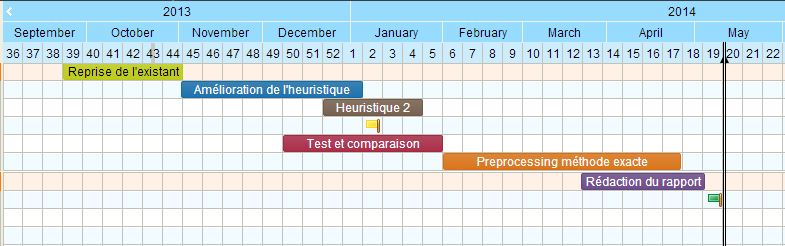
\includegraphics{pics/gantt.jpg}
	\caption{Diagramme de Gantt}
	\label{fig:gantt}
\end{figure}
\bigskip

\section{Gestion de versions}
Le système de gestion de versions Git a été mis en place pour sauvegarder tous les programmes et les données de tests. A la fin du projet, il y a 137 commits soumis au total. La version finale des programmes peut être trouvée sur la plateforme Redmine de l'école. Un paquet qui contient toutes les données du projet est aussi livré.

